\section{Database annotation errors} \label{sec:Clustering_Anomalies}

To evaluate the anomalies in \autoref{fig:PCA_Cluster_Knee_4} \textbf{\textsf{B}} and \textbf{\textsf{C}}, an evolutionary distance was calculated by \gls{MSA} for every eventually misplaced sequence (\autoref{sec:MAFFT}). Therefore, the eventually misplaced sequence was compared to ten other sequences. A sample of five sequences from the same cluster related to the dominant subtype of the cluster, and a sample of five sequences with subtype equal to the misplaced sequence but from other clusters. The mean of distances was then calculated for both cases to rate the assignment and reveal possible misannotations in the \gls{IRD}. 

\begin{table}[!hbt]
    \centering
    \caption[Anomalies in segment 4 cluster 2 with PK]{\textbf{Anomalies in segment 4 cluster 2 with PK.} The \glspl{MSA} mean distance of the given sequences in comparison to a sample of H1 sequences of the same cluster and a sample of H10 sequences present in other clusters.}
    \label{tab:PCA_Error_4_2}
    \pgfplotstabletypeset[
        every head row/.style={
            before row={
                \toprule
            },
            after row={
                \midrule
            },
        },
        every last row/.style={
            after row={
                %... & ... & ... & ... & ... & ... & ... & ...\\
                \bottomrule
            },
        },
        begin table=\begin{tabular*}{0.75\textwidth},
        end table=\end{tabular*},
        columns={0,1,2},
        columns/0/.style={string type,multicolumn names=l,column name=\textbf{Accession}, column type=@{\extracolsep{\fill}\hspace{6pt}}l},
        columns/1/.style={multicolumn names=l,column name=\textbf{H1}, column type=l},
        columns/2/.style={multicolumn names=l,column name=\textbf{H10}, column type=l},
    ]
    {PCA/error_segment_4_cluster_2_difference_head.csv}
\end{table}

In case of \autoref{fig:PCA_Cluster_Knee_4} \textbf{\textsf{C}}, a single sequence with subtype H10 was classified as belonging to cluster 2 which other than that completely consists of H1 and unclassified sequences. By investigation on this possible misplacement, comparison with \gls{MSA} was used. The results for this comparison in \autoref{tab:PCA_Error_4_2} points to the fact, that the as H10 annotated sequence with accession MK237334 is related to subtype H1. The mean of evolutionary distance based on \glspl{MSA} with the sequence and a sample of cluster 0 H1 sequences was very low. Considering the large size of cluster 0 a higher difference was expected, pointing in direction of many very similar sequences in the cluster. Nevertheless, the evolutionary distance of the sequence in comparison to a sample of random H10 sequences was much higher (\autoref{tab:PCA_Error_4_2}). %Even when considering the random sampling of the H10 sequences and the possibility of higher differences of the sequences by origination from different clusters, a misannotation is still more likely. 
Furthermore, only this sole sequence, annotated as subtype H10, was present in a cluster of over 900 sequences of H1 with a very low evolutionary distance to a sequence sample of the cluster, rendering the error most likely as a misannotation.

\begin{table}[!hbt]
    \centering
    \caption[Anomalies in segment 4 cluster 48 with PK]{\textbf{Anomalies in segment 4 cluster 48 with PK.} The \glspl{MSA} mean distance of the given sequences in comparison to a sample of H16 sequences of the same cluster and a sample of H13 sequences present in another cluster. Only the first 20 columns are presented here, the full table can be found in the projects GitHub Repository\footnotemark.}
    \label{tab:PCA_Error_4_48}
    \pgfplotstabletypeset[
        every head row/.style={
            before row={
                \toprule
            },
            after row={
                \midrule
            },
        },
        every last row/.style={
            after row={
                ... & ... & ...\\
                \bottomrule
            },
        },
        begin table=\begin{tabular*}{0.75\textwidth},
        end table=\end{tabular*},
        columns={0,1,2},
        columns/0/.style={string type,multicolumn names=l,column name=\textbf{Accession}, column type=@{\extracolsep{\fill}\hspace{6pt}}l},
        columns/1/.style={multicolumn names=l,column name=\textbf{H16}, column type=l},
        columns/2/.style={multicolumn names=l,column name=\textbf{H13}, column type=l},
    ]
    {PCA/error_segment_4_cluster_48_difference_head.csv}
\end{table}

\footnotetext{\url{https://github.com/ahenoch/Masterthesis.git}}
When comparing the distances for the same calculation performed on \autoref{fig:PCA_Cluster_Knee_4} \textbf{\textsf{C}} in \autoref{tab:PCA_Error_4_48}, no decision for misannotation can be made. The dominant subtype in the cluster 48 is H16 but the sequences of subtype H13 that seem to be misplaced in the cluster have a smaller distance to the sample of sequences from subtype H13. The difference in distance to sample sequences of H13 as well as to sequences of H16 gave indeed no clear finding. Both results are quite similar and the misclustered sequences seem to share much sequence similarity with both subtypes. Maybe the misclustered sequences in cluster 48 point to a more complex classification. Cluster 48 remained a mixed cluster with many sequences from subtype H13 and H16 and, thus, was treated as clustering error. Therefore, subtype H13 and H16 are the focus of investigations of the clustering behavior in the following sections to reveal possible subdivisions responsible for the clustering error.

\begin{figure}[!hbt]
    \centering
    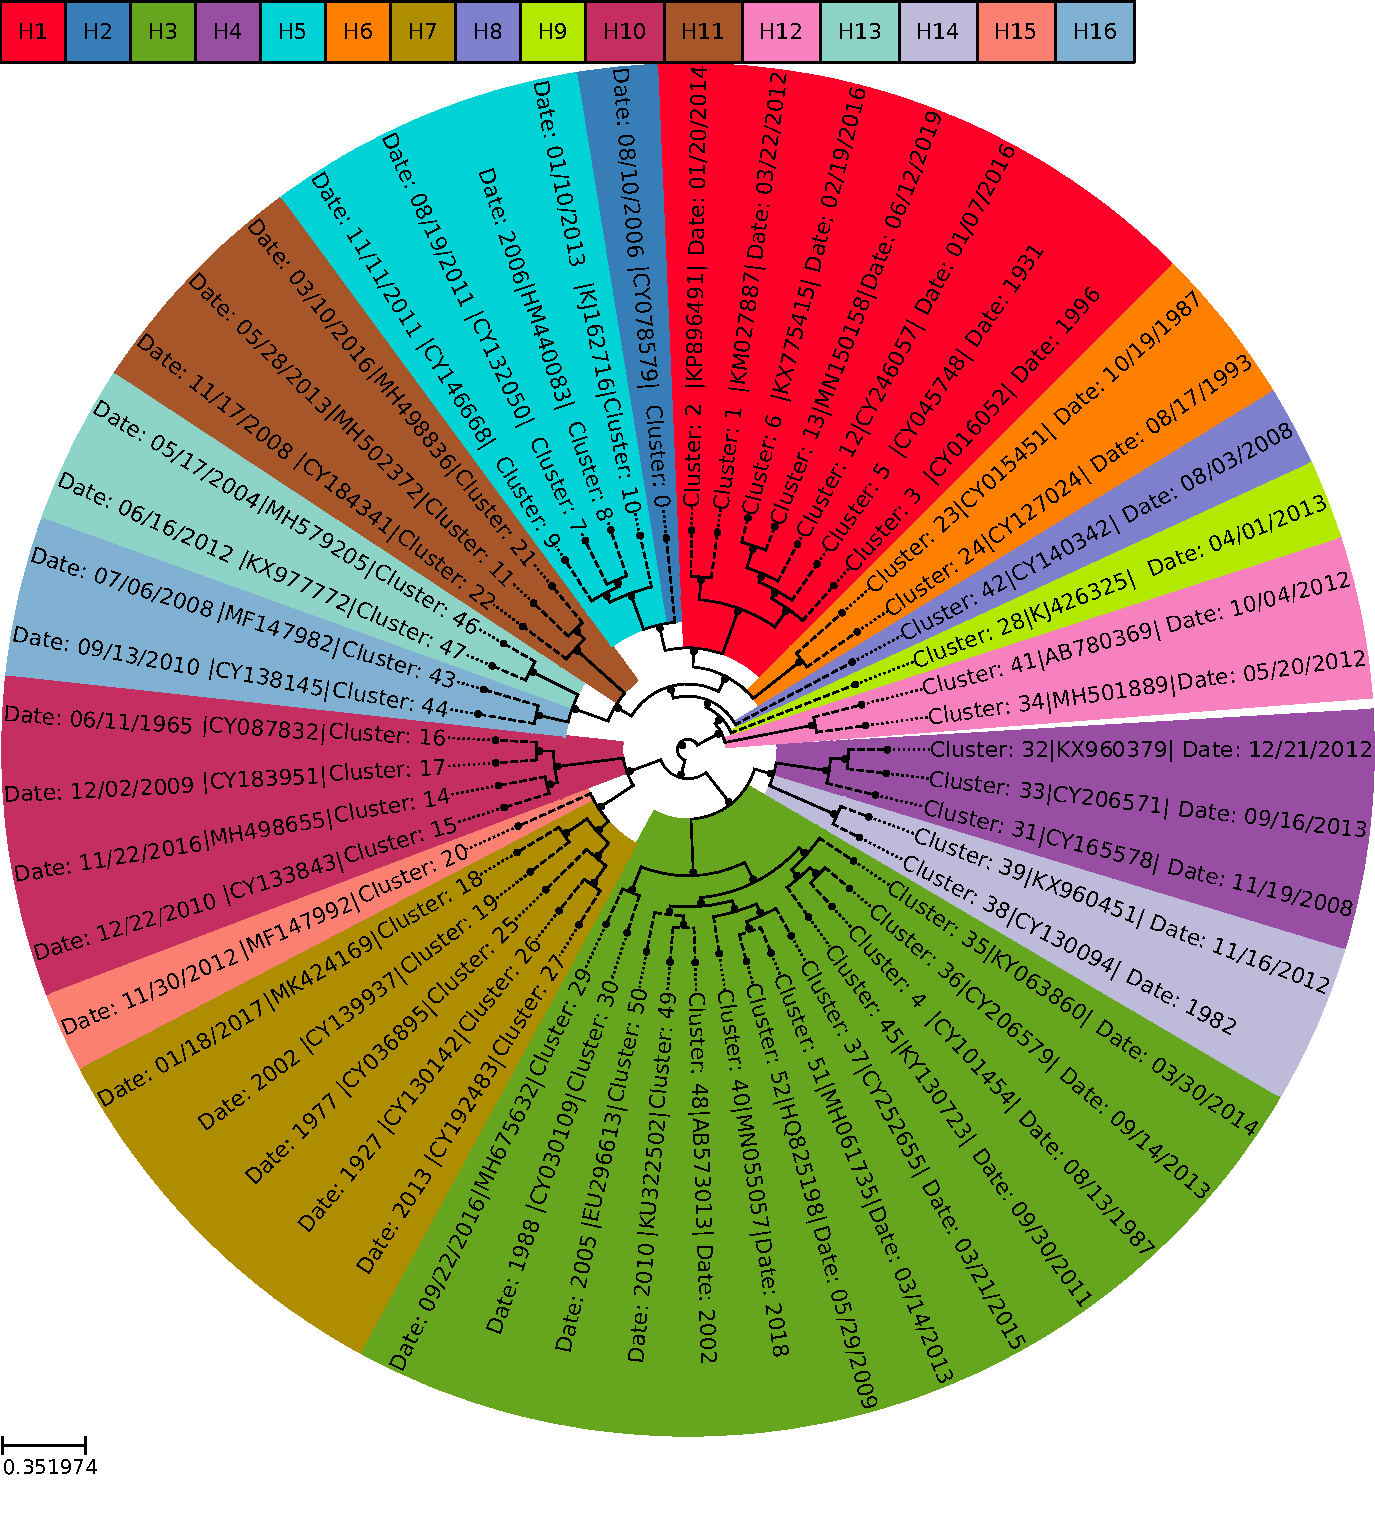
\includegraphics[width=\textwidth]{PCA/Guidetree_segment_4_H_Centroid.pdf}
    \caption[Centroid guidetree of segment 4 with PK]{\textbf{Centroid guidetree of segment 4 with PK.} The guide tree was created by building a \gls{MSA} on the centroid sequences of clusters resulting from the \texttt{PCA} and Kneedle Algorithm (PK) pipeline. The labeling of the tree is based on the related subtype of the centroid sequence used for the \gls{MSA}. The leaves are annotated by the used centroid sequences accession and the cluster it represents.}
    \label{fig:PCA_Guidetree_Centroid_4}
\end{figure}

The last error involved cluster 4, that is homogeneous for subtype H3 but is split off the other H3 clusters by nearly all the non H3 clusters \autoref{fig:PCA_Cluster_Knee_4} \textbf{\textsf{D}}. By evaluation of the clusters relation with a \gls{MSA} created guide tree generated from the centroid vectors sequences, the error persists (\autoref{fig:PCA_Guidetree_Centroid_4}). Every of the 55 clusters have a sequence that should best represent the whole cluster, the centroid sequence, calculated as described in \autoref{sec:MAFFT}. When using the guide tree as comparison, the uniform labeled distribution stood out. Even the centroid of the mentioned cluster 4 is arranged in a line with all the centroids of clusters homogeneous for subtype H3. This subset of centroid sequences used for the guide tree might be to small for a sure proof, but still the centroid sequences should be the most meaningful ones representing the whole cluster and point to a clear subtype separation. Therefore cluster 4 and 48 (\autoref{fig:PCA_Cluster_Knee_4} \textbf{\textsf{C}} and \textbf{\textsf{D}}) remained as identified clustering mistakes and are further examined in the following.

%Übergang zu cluster Comparison durch Centroid Alignment Tree -> H13/H16 Clustertree, Alignmenttree Vergleich -> Cluster H13/H16 Comparison
%fehler im clustering oder fehler in der DAtenbank